\section{Automated System Building with Continuous Integration}
%We want to be assisted in integrating newly developed features etc.
%Also, automate tests (dev env / target) and docs
%Android APK availability
%Hand in hand with agile
While implementing our Android application, it is important that we do not get disconnected from the end product, albeit an unfinished one.
This means that we need some way of continuously integrating new features, bug--fixes, and other changes into the code base, whilst also reflecting them in the product.
However, we still want to have some assurance of our product working as intended, which means that we also need to perform some form of testing.

\bigskip
To meet these needs, we implement a so called \textit{continuous integration} or \textit{CI} into our development process.
This CI includes conducting the following steps in a sandboxed environment, meaning that no state is saved across runs:
\begin{enumberate}
\item checkout the changed code base to be build in two seperate build processes;
\begin{enumberate}
    \item one which continues the build process on the changes code base as is; and
    \item one which merges the changes into the master branch and continues from there;
\end{enumberate}
\item compiling the app and linking dependencies, such as external libraries;
\item linting the newly added code, which entails checking the code style for bad practices and use of deprecated functionality in e.g. the Android APIs;
\item performing tests, both unit testing but also device tests which requires running the application on an actual Android phone;
\item generate documentation, based on the Javadoc\footnote{\url{https://en.wikipedia.org/wiki/Javadoc}} defined in comments throughout the code; and
\item finally, packaging the Android app into a downloadable apk--file, for pre--release distribution.
\end{enumberate}
As described in the sub points \textit{1.1} and \textit{1.2}, the automated build system, effectively carries out two builds for every run, one of the changes in an isolated manner, and one where the changes are integrated with the current master branch.
This ensures that if both processes pass successfully, the new or changed code can be merged into the master branch without compromising the product.

To carry out these tasks we use a piece of software called Jenkins\footnote{\url{https://jenkins.io/}}, which is a build automation server.
The build and build process, our Android app in this case, is then defined in a \textit{Jenkinsfile}, which is a recipe with steps to follow for the Jenkins server.
In our case, the output of the continuous integration using a Jenkins server, are test and linting reports, documentation, and the aforementioned packaged apk--file.

The process of developing on our Android app, is based upon a workflow revolving around source code management using \textit{git}\footnote{\url{https://git-scm.com/}}, and project management using Phabricator\footnote{\url{https://www.phacility.com/}} and the Github\footnote{\url{https://github.com}} feature \textit{pull requests}.
This development process will be further explained and discussed in \cnameref{cha:development_method}.

We set up the continuous integration, such that any pull request and update to the master branch activates the automated build system on a in--house Jenkins server.
This ensures that code, to be merged into the master branch and hereby the current product, will be required to pass the continuous integration process.

The workflow of our Jenkins server can be seen on \cref{fig:jenkins_workflow}, where we have simplified the process for illustration purposes; e.g. the three last steps are executed for each processing, i.e. both the clean run and the one merged with the master branch.
Moreover, the step which includes testing, linting, and generating documentation, should be seen as a parallel process, where the subcomponents are executed in parallel on the server.

\begin{figure}[tb]
    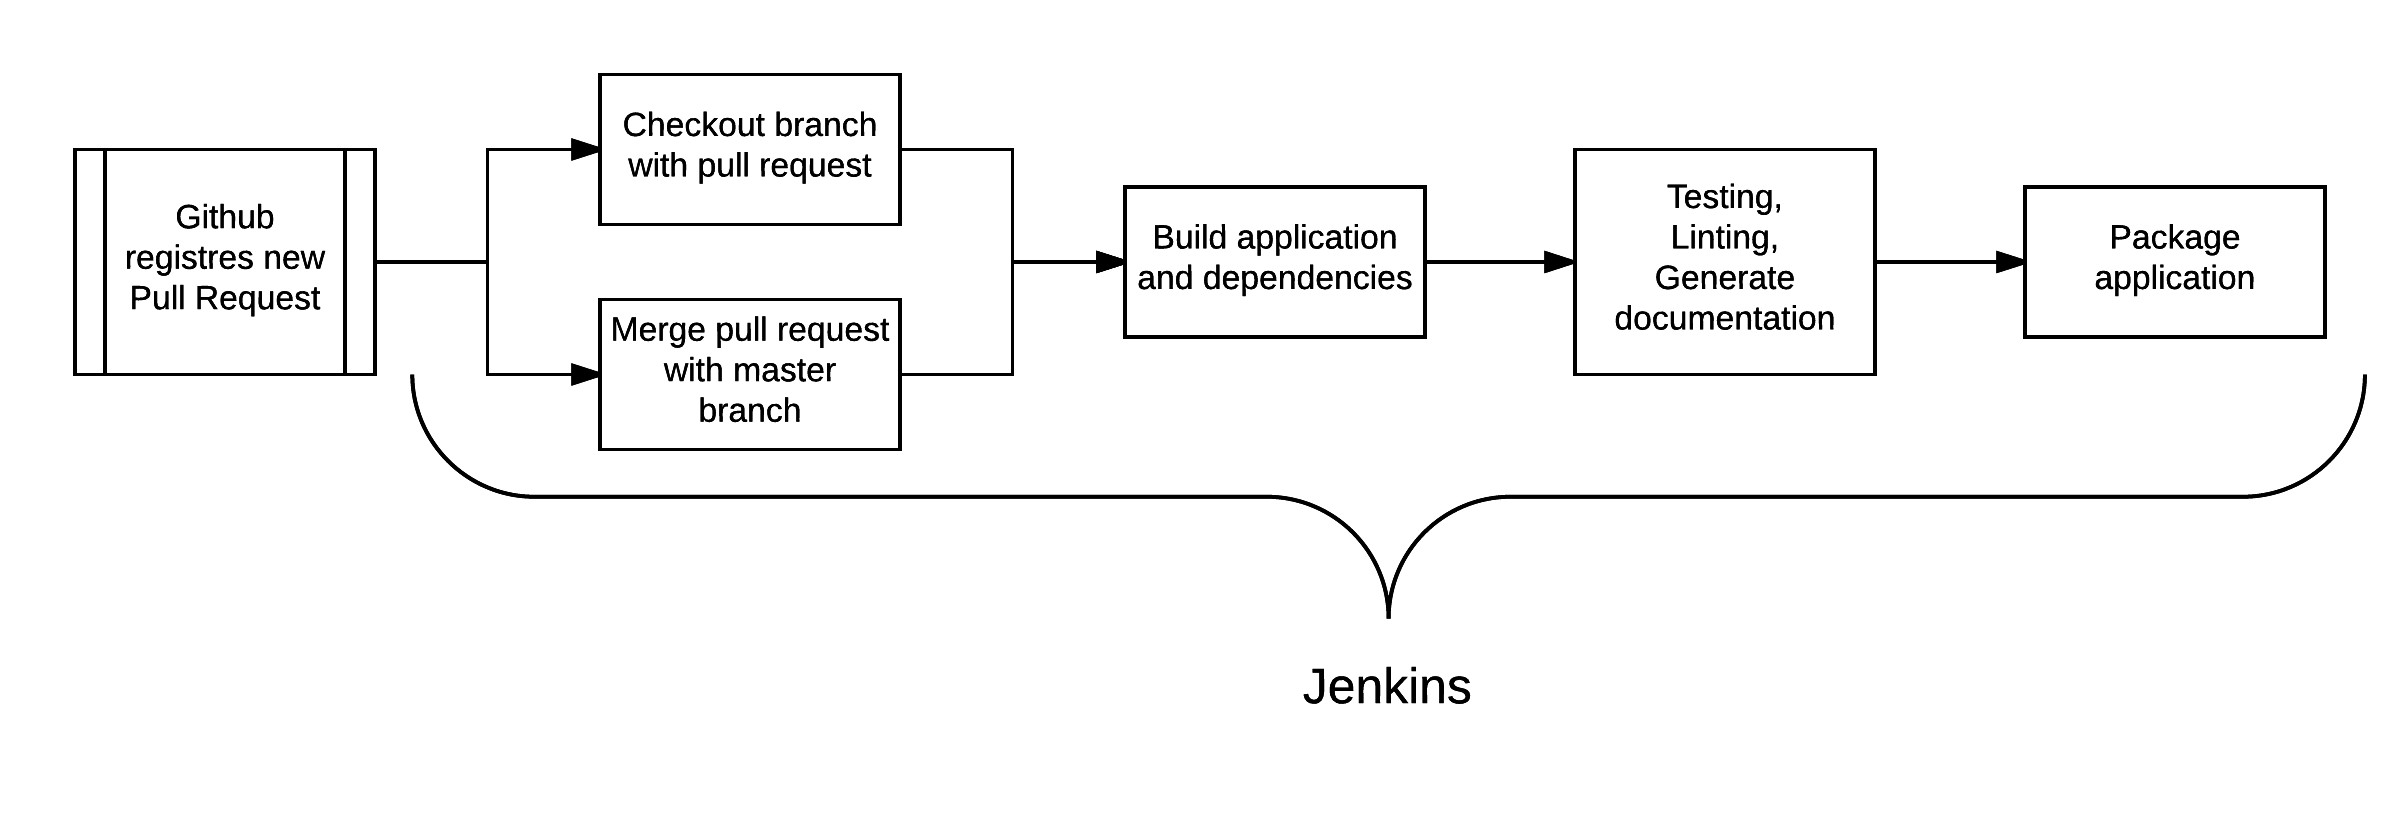
\includegraphics[width=1\textwidth]{./jenkins_workflow.png}
    \caption{Depiction of the workflow of our automated build system}\label{fig:jenkins_workflow}
\end{figure}

A consequence of the automated build system, is then that when a developer reviews new or changed code in pull request, they are assisted by the linting and tests reports, and are furthermore able to quickly try out the application by downloading and installing the packaged apk on their own device.

\bigskip
Another benefit to the continuous integration and automated build system, we set up, is that it also backs up an agile development process, especially since all updated to the master branch, are presented as a ready--to--use product in the form of a downloadable apk.

In a future iteration, one could even integrate continuous deployment in the automated build system, such that all approved changes to the master branch would be pushed directly to a distribution platform such as Google Play.

